\chapter{Mesterséges intelgiencia betanítása és használata}
\thispagestyle{fancy}
\pagestyle{fancy}


A célom az, hogy a mesterséges intelgiencia játéka, amit használni fogok, a lehető legjobban hasonlítson az emberi gondolkodáshoz. Az emberi agy működéséhez a legjobban 
a neurális hálózat hasonlítható, így ezt fogom én is használni a projektemhez. 



\section{Tensorflow}
Terveim szerint, python nyelven akartam elkészíteni az MI. tanításához az algoritmust. Ehhez a legjobbnak a TensorFlow-t \cite{tensorflow2015-whitepaper} találtam. A TensorFlow weboldalán ingyenesen elérhető dokumentációkból és tanító anyagokból  könnyedén ki tudtam indulni. 

A dokumentáció szerint, minden felhasználónak alapvetően a Keras API használatát javasolják, így hát én is azt használtam. 

\section{Tervezés}
Az elképzelésem szerint, egy Sequential, azaz szekvenciális modelt használok. A szekvenciális modelben pontosan egyetlen bemeneti tensor és egyetlen kimeneti tensor található. 

Az én esetemben a bemeneti tensor a játék jelenlegi állása, a kimenet pedig a következő felfordítandó kártya lesz. Mivel a tensornak a típusa nem változik, pusztán az értéke, ezért nekem ez tökéletesen megfelelő. 

A modelt be kell tanítanom a gyüjtött adatokkal. Ehhez a legegyszerűbb, ha az adataimat egy JSON file-ba összefűzöm, így a scriptnek elég ezt az egy file-t beolvasnia. 

Minél jobban le tudom egyszerűsíteni a bemeneti rétegem, úgy, hogy a lehetőleg ne legyen benne adatvesztés, annál gyorsabban véghez tudom vinni a tanítást. 
Ha bonyolult az input layer, akkor a tanulás lelassul, és számomra fontos perceket, órákat, de akár napokat is veszíthetek, egy hibás model esetén. 

Példának okért, tegyük fel, hogy nem tarnszformálom át a gyüjtött adatoka és a játék $N$ lépésből áll. Mivel mind az $N$ esetben, az előző $N-1$ lépést is oda kell adnom a tanító algoritmusnak, és 1.-től $N$-dik lépésig az összes lépést megtanítom a modelnek, így 
egy $N$ lépésből álló játéknak a tanításhoz felhasznált adatmennyisége:

\[\frac{N(N+1)}{2} = \frac{N^2+N}{2}\]

Tehát látható, hogy exponenciálisan nő az adatok mennyisége. Annak érdekében, hogy ezt elkerüljem, a következő ötlettel áltam elő:

A hash-függvényeket az informatikában az 1980-as évek óta alkalmazzák arra, hogy bármilyen méretű adatot rögzített hosszúságúra alakítsanak át. Gyakorlati felhasználási területük például a fájlok ellenőrzése, mivel ha két fájl tartalma teljesen megegyezik, akkor az azokból képzett hash is azonos lesz. Ez különösen hasznos, amikor dokumentumokat töltünk fel egy fájlszerverre, mivel így könnyen ellenőrizhető, hogy a fájl már létezik-e a szerveren, és elkerülhető a duplikált tárolás.

A hash-függvények segítségével, képes lehetek minden lépést és az őt megelőző összes eddigi lépés eggyüttesét  fix hosszú bit vektorrá alakítom, így szignifikáns mennyiségű adatmennyiséget tudok spórólni. 
Természetesen így lehetségessé válik, hogy nem lesz teljesen pontos a betanított modellem, azonban ez a kockázat minden transzformáció esetén előfordulhat. 

\begin{figure}[h]
    \centering
    \begin{adjustbox}{width=0.75\textwidth}
        \label{diagram:deepLearningModel}  
        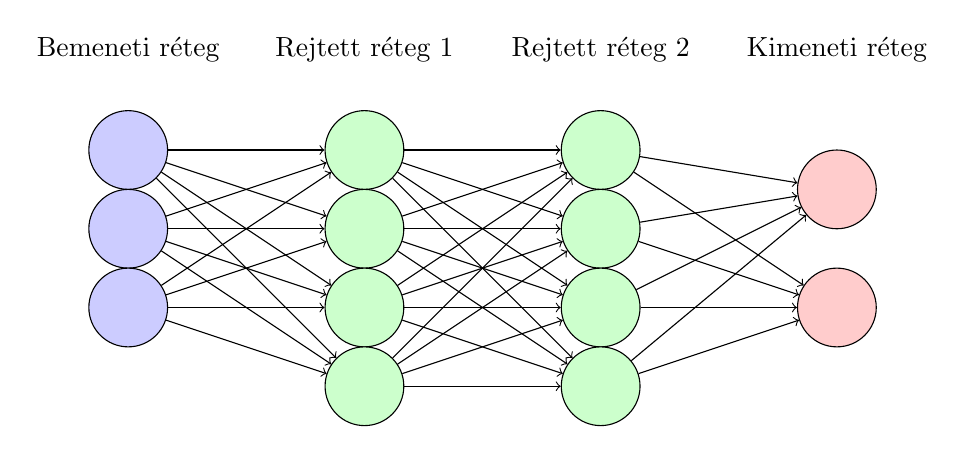
\begin{tikzpicture}[
            node distance=1.5cm and 2cm,
            input neuron/.style={circle, draw, fill=blue!20, minimum size=1cm},
            hidden neuron/.style={circle, draw, fill=green!20, minimum size=1cm},
            output neuron/.style={circle, draw, fill=red!20, minimum size=1cm},
            neuron missing/.style={draw=none, fill=none, text height=0.5cm, execute at begin node=\color{black}$\vdots$}
        ]
        
        % Input layer
        \foreach \m in {1,2,3}
            \node[input neuron] (I-\m) at (0,-\m) {};
        
        % Hidden layer 1
        \foreach \m in {1,2,3,4}
            \node[hidden neuron] (H1-\m) at (3,-\m) {};
        
        % Hidden layer 2
        \foreach \m in {1,2,3,4}
            \node[hidden neuron] (H2-\m) at (6,-\m) {};
        
        % Output layer
        \foreach \m in {1,2}
            \node[output neuron] (O-\m) at (9,-1.5*\m) {};
        
        % Connect input layer to hidden layer 1
        \foreach \i in {1,2,3}
            \foreach \j in {1,2,3,4}
                \draw[->] (I-\i) -- (H1-\j);
        
        % Connect hidden layer 1 to hidden layer 2
        \foreach \i in {1,2,3,4}
            \foreach \j in {1,2,3,4}
                \draw[->] (H1-\i) -- (H2-\j);
        
        % Connect hidden layer 2 to output layer
        \foreach \i in {1,2,3,4}
            \foreach \j in {1,2}
                \draw[->] (H2-\i) -- (O-\j);
        
        % Labels
        \node[above] at (0,0) {Bemeneti réteg};
        \node[above] at (3,0) {Rejtett réteg 1};
        \node[above] at (6,0) {Rejtett réteg 2};
        \node[above] at (9,0) {Kimeneti réteg};
        
        \end{tikzpicture}
    \end{adjustbox}
    \caption{Neurális háló, egy bemeneti két rejtett és egy kimeneti réteggel}
\end{figure}

\section{Adatok transformálása}

Az adatok transformálását a program futása közben, felhasználás előtt készítem elő. Ez azért lesz hasznos, mivel a játék közben, a kész model felhasználásakor is dinamikusan kell az adatokat hash-függvénnyel leképeznem.

\begin{itemize}
    \item Beolvasom a JSON állományt. 
    \item Végigmegyek az adatokon, és létrehozok egy szöveges változót. Ez a változó tartalmazza a JSON-ban található aktuális és az összes előző lépést  (\ref{code:json_to_hash}. ábra). 
    \item A python hashlib csomagja segítségével ezt a változót leképezem az SHA256 függvényt használva egy hexadecimális stringgé. 
    \item A leképezett hexadecimális stringet tovább transzformálom. 
    Végigmegyek az összes karakterén, minden karakter egy hexadecimális szám. Ezen számokat leképezem egy decimális számmá, majd tovább konvertálom egy 4 bit hosszú binárissá. Ezen 4 számjegyű számokat összefűzöm egy stringgé, majd átkonvertálom, hogy egy darab 256 bitből álló NumPy tömböt kapjak, melyet fel fogok tudni használni a tanításhoz (\ref{code:hash_to_bit}. ábra). 
\end{itemize}

\begin{figure}[h]
    \includegraphics[width=0.75\textwidth]{img/JSON_TO_SHA256.png}
    \caption{Kód részlet, amely leképezi a $key$ által megadott játék lépéseit egy hash tömbbé. A hash-ek mellett a következő lépéssel tér vissza.}
    \label{code:json_to_hash}
\end{figure}

\begin{figure}[h]
    \includegraphics[width=0.75\textwidth]{img/hash_to_bit.png}
    \caption{Kód részlet. Az SHA256 hash hexadecimális string bitsorozattá konvertálása.}
    \label{code:hash_to_bit}
\end{figure}

\section{A tanító algoritmus}

A TensorFlow része a Keras API, mely segítségével könnyedén és egyszerűen létre tudok hozni szekvenciális modelt (\ref{code:tensor}. ábra). A model bemeneti rétege egy 256 nagyságú tömböt vár, melyben bitek találhatók. 

A következő két réteghez egy 128 és egy 64 neuront tartalmazó teljesen kapcsolodó (Dense) réteget használok. Dense layer azt jelenti, hogy a réteg összes neuronja kapcsolodik az előző réteg összes neuronjával. Ez a neuron típus gyarkan használt előre csatolt neurális hálóknál. Az aktivációs függvény amit ezekhez a rétegekhez használok az az úgynevezett ReLU(Rectified Linear Unit) függvény, mely a következő képpen néz ki: 
\ 
\begin{figure}[h]
    \includegraphics[width=0.75\textwidth]{img/Tensor.png}
    \caption{Kód részlet. A tanító algoritmus}
    \label{code:tensor}
\end{figure}